\documentclass[11pt,a4paper]{article}

\usepackage[margin=25mm]{geometry}
\usepackage{amsmath, amssymb, amsthm}
\usepackage{physics}       % \dd, \grad, \curl, \div, bra-ket
\usepackage{bm}            % \bm{} for bold-italic vectors
\usepackage{siunitx}       % \SI{3e8}{\meter\per\second}
\usepackage{booktabs}      % \toprule \midrule \bottomrule
\usepackage{array}
\usepackage{graphicx}
\graphicspath{{./figs/}}
\usepackage{tikz}
\usepackage{algorithm}
\usepackage{algpseudocode}
\usepackage{hyperref}      % LAST package

\newcommand{\abar}{\bar{a}}
\newcommand{\Df}{D_\text{f}}
\newcommand{\kf}{k_\text{f}}
\newcommand{\RF}{R_\text{F}}
\newcommand{\Rg}{R_\text{g}}
\newcommand{\dmin}{\delta_\text{min}}
\newcommand{\dmax}{\delta_\text{max}}
\newcommand{\nSA}{n_\text{SA}}

\title{Theory note: PTSA and tunable CCA aggregate generators\\
\large aggregate\_generator\_PTSA v0.5.0}
\author{Nobuhiro Moteki}
\date{\today}

\begin{document}
\maketitle

\begin{abstract}
This note describes the two algorithms implemented in aggregate\_generator\_PTSA.
Both build aggregates of non-overlapping spheres in point contact.
Both are tuned by a fractal prefactor $\kf$ and a fractal dimension $\Df$.
The polydisperse tunable sequential aggregation (PTSA) adds one monomer at a time.
The tunable cluster-cluster aggregation (TCCA) merges clusters pairwise.
We state the placement laws as implemented in the code and derive them from one exact identity for the radius of gyration.
We also document how the TCCA code extends the original C++ implementation and compare the two methods at equal $(\kf, \Df)$.
\end{abstract}

\tableofcontents

%======================================================================
\section{Common definitions}
\label{sec:common}

\subsection{Monomers}
\label{sec:monomers}

An aggregate consists of $N_\text{p}$ spherical monomers.
Monomer $i$ has centre $\bm{r}_i$ and radius $a_i$.
Lengths are in \si{\micro\meter} in the code.
All formulas below are scale invariant, so any length unit works.

The radii are independent draws from a normal distribution clipped at $\pm 2$ standard deviations:
\begin{equation}
  a_i = \abar\,(1 + \sigma_a z_i), \qquad
  z_i = \max\!\bigl(-2, \min(2, \sqrt{-2\ln u_{1,i}}\,\cos 2\pi u_{2,i})\bigr),
  \label{eq:radius-distribution}
\end{equation}
where $\abar$ is the mean radius (\texttt{mean\_rp}), $\sigma_a$ is the relative standard deviation (\texttt{rel\_std\_rp}), and $u_{1,i}, u_{2,i}$ are uniform random numbers on $[0, 1)$.
The Box--Muller transform gives $z_i$.
Both generators use this distribution.

Each monomer has mass $m_i = (4\pi/3)\rho a_i^3$.
The density $\rho$ cancels in every formula, and the code uses $\rho = 1$.
The centroid of a set $S$ of monomers is mass weighted:
\begin{equation}
  M_S = \sum_{i \in S} m_i, \qquad
  \bm{r}_{\text{c},S} = \frac{1}{M_S} \sum_{i \in S} m_i \bm{r}_i .
  \label{eq:centroid}
\end{equation}
Both generators keep the centroid of the growing cluster at the origin.

\subsection{Radius of gyration}
\label{sec:rg}

Two definitions of the radius of gyration appear in this note.
They differ only in the self term of each monomer.

The \emph{Filippov radius} $\RF$ is used inside the placement laws.
Its self term is $a_i^2$, as in Filippov et al.~\cite{filippov2000}:
\begin{equation}
  \RF^2(S) = \frac{1}{M_S} \sum_{i \in S} m_i \left( \abs{\bm{r}_i - \bm{r}_{\text{c},S}}^2 + a_i^2 \right).
  \label{eq:rg-filippov}
\end{equation}
For equal radii $a_i = a$ this is $\RF^2 = a^2 + \langle \abs{\bm{r} - \bm{r}_\text{c}}^2 \rangle$.
This is Eq.~[4] of Ref.~\cite{filippov2000} and the definition of the C++ code~\cite{moteki2019}.
Filippov et al.\ chose it because it gives $\RF = a$ for a single sphere.

The \emph{output radius} $\Rg$ is stored in the HDF5 files and catalogs for both methods.
Its self term is the moment of inertia of a solid sphere, $(3/5)a_i^2$:
\begin{equation}
  \Rg^2 = \frac{1}{M} \sum_{i} m_i \left( \abs{\bm{r}_i - \bm{r}_\text{c}}^2 + \frac{3}{5} a_i^2 \right).
  \label{eq:rg-output}
\end{equation}
The derived quantities are
\begin{equation}
  R_\text{e} = \sqrt{5/3}\,\Rg, \quad
  V_\text{agg} = \frac{4\pi}{3} R_\text{e}^3, \quad
  V = \sum_i \frac{4\pi}{3} a_i^3, \quad
  R_\text{ve} = \left( \frac{3V}{4\pi} \right)^{1/3}, \quad
  P_\text{agg} = 1 - \frac{V}{V_\text{agg}} ,
  \label{eq:derived}
\end{equation}
where $P_\text{agg}$ is the porosity (\texttt{eps\_agg} in the code) by the gyration method.

\subsection{Fractal scaling law}
\label{sec:fractal-law}

A cluster of $N$ monomers obeys the fractal law when
\begin{equation}
  N = \kf \left( \frac{\RF}{a} \right)^{\Df} ,
  \qquad\text{i.e.}\qquad
  \RF^2 = a^2 \left( \frac{N}{\kf} \right)^{2/\Df} ,
  \label{eq:fractal-law}
\end{equation}
where $a$ is a monomer length scale.
For equal radii $a$ is the monomer radius.
Section~\ref{sec:polydisperse} discusses the choice of $a$ for polydisperse monomers.
The code calls the prefactor \texttt{k}.

\subsection{Two-body identity}
\label{sec:identity}

Both placement laws follow from one exact identity.
Let cluster~1 have mass $M_1$, centroid $\bm{r}_{\text{c},1}$, and Filippov radius $R_{\text{F},1}$.
Let cluster~2 have $M_2$, $\bm{r}_{\text{c},2}$, and $R_{\text{F},2}$.
Let $\Gamma = \abs{\bm{r}_{\text{c},1} - \bm{r}_{\text{c},2}}$ and $M = M_1 + M_2$.
The merged centroid is $\bm{r}_\text{c} = (M_1 \bm{r}_{\text{c},1} + M_2 \bm{r}_{\text{c},2})/M$.
Inserting $\bm{r}_i - \bm{r}_\text{c} = (\bm{r}_i - \bm{r}_{\text{c},1}) + (\bm{r}_{\text{c},1} - \bm{r}_\text{c})$ into Eq.~\eqref{eq:rg-filippov} makes the cross terms vanish, because each cluster is centred on its own centroid.
The result is
\begin{equation}
  \RF^2 = \frac{M_1 R_{\text{F},1}^2 + M_2 R_{\text{F},2}^2}{M}
        + \frac{M_1 M_2}{M^2}\,\Gamma^2 .
  \label{eq:parallel-axis}
\end{equation}
We require the merged cluster to have a prescribed radius $R_\text{t}$.
Solving Eq.~\eqref{eq:parallel-axis} for $\Gamma$ gives
\begin{equation}
  \Gamma^2 = \frac{M^2}{M_1 M_2} R_\text{t}^2
           - \frac{M}{M_2} R_{\text{F},1}^2
           - \frac{M}{M_1} R_{\text{F},2}^2 .
  \label{eq:gamma-general}
\end{equation}
For equal spheres Eqs.~\eqref{eq:parallel-axis} and~\eqref{eq:gamma-general} are Eqs.~[13] and~[14] of Ref.~\cite{filippov2000}.
Equation~\eqref{eq:parallel-axis} contains no orientation.
Any rotation of either cluster about its own centroid leaves $\RF$ unchanged.
Placing the centroids at distance $\Gamma$ therefore fixes $\RF$ of the merged cluster exactly, whatever the orientations.
A real solution requires $\Gamma^2 > 0$.

\subsection{Contact criteria}
\label{sec:contact}

The surface gap of monomers $i$ and $j$ is
\begin{equation}
  g_{ij} = \abs{\bm{r}_i - \bm{r}_j} - (a_i + a_j) .
  \label{eq:gap}
\end{equation}
A trial configuration is \emph{overlapping} if any pair has $g_{ij} < \dmin$.
It is \emph{attached} if it does not overlap and at least one pair has $g_{ij} < \dmax$.
Both codes use $\dmin = 10^{-6}\,\abar$ as a numerical safety margin.
The contact window $\dmax$ differs between the methods (Secs.~\ref{sec:ptsa-search} and~\ref{sec:tcca-merge}).

A random direction $\hat{\bm{e}}$ is drawn uniformly on the unit sphere as
\begin{equation}
  \hat{\bm{e}} = \left( \sqrt{1-u^2}\cos\phi,\ \sqrt{1-u^2}\sin\phi,\ u \right), \qquad
  \phi = 2\pi u_1, \quad u = 2u_2 - 1 .
  \label{eq:random-direction}
\end{equation}

%======================================================================
\section{PTSA: polydisperse tunable sequential aggregation}
\label{sec:ptsa}

PTSA is a particle-cluster method.
Monomers are added one at a time to a single growing cluster.
Singh and Tsotsas introduced the tunable sequential aggregation for monodisperse monomers~\cite{singh2020}.
They extended it to polydisperse monomers~\cite{singh2021,singh2022}.
The idea of tuning both $\kf$ and $\Df$ through the radius of gyration goes back to Filippov et al.~\cite{filippov2000}.
The equations below are those of the implementation in this repository.
The placement distance~\eqref{eq:ptsa-distance} is Eq.~(2) of Ref.~\cite{singh2022}.
The tuned dimension in the second case of Eq.~\eqref{eq:ptsa-tuned-dimension} is Eq.~(1) of Ref.~\cite{singh2022}, where it is attributed to Ref.~\cite{singh2020}.
Singh derives it in his thesis (Eqs.~(4.8)--(4.10) of Ref.~\cite{singh2021thesis}).
The first case of Eq.~\eqref{eq:ptsa-tuned-dimension} is the limit of Eq.~(4.12) of the same thesis.
The contact window~\eqref{eq:ptsa-window} appears in none of Refs.~\cite{singh2021,singh2021thesis,singh2022}.
It belongs to this implementation.

Singh and Tsotsas also proposed a modified algorithm (MPTSA)~\cite{singh2021}.
It uses the individual monomer masses in the placement distance.
It also replaces the self term $a^2$ by the solid-sphere value $0.6\,a^2$, because they regard the Filippov self term as an error.
The function \texttt{ptsa} in this repository implements the earlier PTSA of Ref.~\cite{singh2022}, not MPTSA.
The choice of self term changes the meaning of $\kf$, so prefactors obtained with the two conventions are not directly comparable.

\subsection{Placement distance}
\label{sec:ptsa-distance}

The first monomer sits at the origin.
The second sits at distance $a_1 + a_2 + \dmin$ in a random direction.
The pair is then shifted so that its centroid is at the origin.

Monomer $n \ge 3$ with radius $a_n$ is placed at distance $R_n$ from the centroid of the first $n-1$ monomers.
The code uses
\begin{equation}
  R_n^2 = \frac{n^2 a_n^2}{n-1}\, n^{2/D'}
        - \frac{n a_n^2}{n-1}
        - n a_n^2 (n-1)^{2/D'} ,
  \label{eq:ptsa-distance}
\end{equation}
with the tuned dimension
\begin{equation}
  D' =
  \begin{cases}
    3 & \text{if } n \le \kf^{3/(3-\Df)}, \\[2pt]
    \Df \dfrac{\ln N_\text{p}}{\ln(N_\text{p}/\kf)} & \text{otherwise}.
  \end{cases}
  \label{eq:ptsa-tuned-dimension}
\end{equation}
The tuned dimension keeps $\RF$ of the final aggregate unchanged when the prefactor is set to~1.
Singh obtained it by equating the porosity at $(\kf, \Df)$ with that at $(1, D')$ for the same $N_\text{p}$~\cite{singh2021thesis}.
For $\kf > 1$ it gives $D' > \Df$.
It exceeds 3, which is not feasible, when $N_\text{p} < \kf^{3/(3-\Df)}$.
Singh therefore builds the first $\kf^{3/(3-\Df)}$ monomers with $D' = 3$~\cite{singh2021thesis}, which is the first case.
For $\kf < 1$ the first case never occurs.

Equation~\eqref{eq:ptsa-distance} is Eq.~\eqref{eq:gamma-general} under three simplifications.
All monomers are treated as having the radius $a_n$ of the new one, so $M_1/M_2 = n-1$.
Singh and Tsotsas state this equal-mass assumption explicitly and note that it follows Skorupski et al.~\cite{skorupski2014}.
The previous cluster is assigned its target radius $R_{\text{F},1}^2 = a_n^2 (n-1)^{2/D'}$, not its measured one.
The target of the new cluster is $R_\text{t}^2 = a_n^2 n^{2/D'}$.
This is the fractal law~\eqref{eq:fractal-law} with prefactor~1 and dimension $D'$.

At the final size the tuned dimension gives
\begin{equation}
  N_\text{p}^{1/D'} = \left( \frac{N_\text{p}}{\kf} \right)^{1/\Df} ,
  \label{eq:ptsa-final}
\end{equation}
so the final aggregate targets $N_\text{p} = \kf (\RF/a)^{\Df}$.
At an intermediate size $n$ the law $n = (\RF/a)^{D'}$ corresponds to the prefactor
\begin{equation}
  k_\text{eff}(n) = \frac{n}{(\RF/a)^{\Df}} = n^{1 - \Df/D'} = \kf^{\ln n / \ln N_\text{p}} .
  \label{eq:ptsa-local-prefactor}
\end{equation}
The prefactor therefore moves from 1 at $n = 1$ to $\kf$ at $n = N_\text{p}$.
PTSA imposes $(\kf, \Df)$ on the final aggregate only.

\subsection{Random search}
\label{sec:ptsa-search}

The candidate position is $R_n \hat{\bm{e}}$ with $\hat{\bm{e}}$ from Eq.~\eqref{eq:random-direction}.
It is tested against all $n-1$ placed monomers.
The test stops at the first overlapping pair.
The first attached candidate is accepted, and the cluster is shifted back to a zero centroid.
The search allows at most \texttt{max\_search} candidates per monomer (default $10^8$).
If none is accepted, the run stops and returns $N_\text{final} = n - 1 < N_\text{p}$.

The PTSA contact window depends on $\Df$ and on the growth stage:
\begin{equation}
  \dmax(n) = \abar\,\tau \left( 1 + 5\,\frac{n-1}{N_\text{p}}\,\frac{2.95 - \Df}{0.6} \right), \qquad
  \tau = 0.001 + 0.0033\,(2.95 - \Df) .
  \label{eq:ptsa-window}
\end{equation}
For $\Df = 2.35$ the window grows from $0.003\,\abar$ to $0.018\,\abar$ during growth.
For $\Df = 2.95$ it is fixed at $0.001\,\abar$.

%======================================================================
\section{TCCA: tunable cluster-cluster aggregation}
\label{sec:tcca}

Thouy and Jullien introduced cluster-cluster aggregation with a prescribed fractal dimension~\cite{thouy1994}.
Their model joins equal clusters at the centre-to-centre distance required by the target scaling.
Filippov et al.\ formulated the off-lattice version that prescribes both $\kf$ and $\Df$~\cite{filippov2000}.
The code \texttt{tcca.py} translates the C++ program \texttt{aggregate\_gen}~\cite{moteki2019} into Python with Numba.
Small initial clusters are built by sequential aggregation (SA).
They are then merged pairwise up a binary hierarchy.
Every merge enforces the fractal law~\eqref{eq:fractal-law} exactly.

\subsection{Hierarchy}
\label{sec:tcca-hierarchy}

Thouy and Jullien merged clusters of equal size, so the final size was a power of~2~\cite{thouy1994}.
Filippov et al.\ allowed clusters of unequal size, so that the final size need not be a power of~2~\cite{filippov2000}.
They started from SA clusters of 5--8 monomers.
The C++ code builds $2^L$ SA clusters of $\nSA$ monomers each (default $\nSA = 4$) and merges equal pairs $L$ times.
It is therefore restricted to $N_\text{p} = \nSA\,2^L$.
The Python code returns to the general scheme of Filippov et al.\ and splits recursively.
A cluster of $N > \nSA$ monomers is built from clusters of $\lfloor N/2 \rfloor$ and $\lceil N/2 \rceil$ monomers.
A cluster of $N \le \nSA$ monomers is built by SA.
Figure~\ref{fig:hierarchy} shows an example.
For $N_\text{p} = \nSA\,2^L$ the result is the C++ hierarchy.
Equation~\eqref{eq:gamma-general} holds for unequal masses, so unequal halves need no change in the formulas.
The operations are executed in post-order, so both children exist before they are merged.
Monomer indices are assigned to contiguous ranges, so the order of rows in the output follows the hierarchy.

\begin{figure}[htbp]
  \centering
  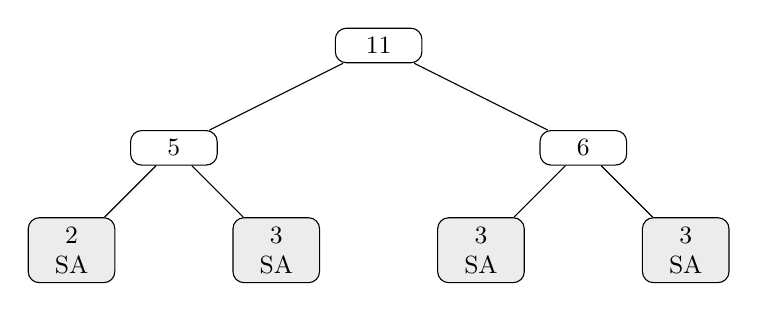
\begin{tikzpicture}[
      level distance=13mm,
      level 1/.style={sibling distance=52mm},
      level 2/.style={sibling distance=26mm},
      every node/.style={draw, rounded corners, minimum width=11mm, align=center, font=\small},
      sa/.style={fill=gray!15}]
    \node {11}
      child {node {5}
        child {node[sa] {2\\SA}}
        child {node[sa] {3\\SA}}}
      child {node {6}
        child {node[sa] {3\\SA}}
        child {node[sa] {3\\SA}}};
  \end{tikzpicture}
  \caption{Hierarchy for $N_\text{p} = 11$ and $\nSA = 4$.
  Shaded leaves are SA clusters.
  Each inner node is a merge of its two children.}
  \label{fig:hierarchy}
\end{figure}

\subsection{Length scale for polydisperse monomers}
\label{sec:polydisperse}

The C++ code treats equal radii only.
The Python code extends it to the distribution~\eqref{eq:radius-distribution}.
Morán et al.\ proposed FracVAL, a tunable CCA for polydisperse monomers that accounts for the individual masses~\cite{moran2019}.
The extension here was derived independently from Eq.~\eqref{eq:gamma-general}.
We have not compared it with FracVAL.
Centroids and $\RF$ are mass weighted as in Sec.~\ref{sec:common}.
The length scale of a cluster $S$ is its mass-weighted rms monomer radius,
\begin{equation}
  a_\text{c}^2(S) = \frac{1}{M_S} \sum_{i \in S} m_i a_i^2 ,
  \label{eq:length-scale}
\end{equation}
and the target radius of a cluster of $N$ monomers is
\begin{equation}
  R_\text{t}^2(S) = a_\text{c}^2(S) \left( \frac{N}{\kf} \right)^{2/\Df} .
  \label{eq:tcca-target}
\end{equation}
With this choice $\RF^2 = a_\text{c}^2 + \langle \abs{\bm{r} - \bm{r}_\text{c}}^2 \rangle_m$, which has the same form as the C++ definition.
Scaling all radii by a factor $\lambda$ scales every placement distance by $\lambda$.
For equal radii $a_\text{c} = a$, and all formulas reduce to the C++ ones.

A fixed length scale $a = \abar$ is not scale consistent.
It makes small SA clusters impossible to build when their monomers are larger than the mean.
For example, take radii $(1.08, 1.11, 1.20)\,\abar$ with $\kf = 0.95$ and $\Df = 2.5$.
With $a = \abar$ the third monomer must sit at $\Gamma = 1.88\,\abar$ from the centroid of the dimer.
On that sphere it overlaps one of the dimer monomers in every direction.

\subsection{Initial clusters by sequential aggregation}
\label{sec:tcca-sa}

An SA cluster starts as in PTSA.
One monomer sits at the origin and the second touches it at gap $\dmin$ in a random direction.
The C++ code places the dimer along the $x$ axis.
This difference has no effect because every cluster is later rotated at random.

Monomer $N \ge 3$ of the cluster is placed at distance $\Gamma_N$ from the centroid of the first $N-1$ monomers.
Equation~\eqref{eq:gamma-general} with cluster~1 being the first $N-1$ monomers and cluster~2 being the new monomer gives
\begin{equation}
  \Gamma_N^2 = \frac{M^2}{M_1 m_N} R_\text{t}^2(N)
             - \frac{M}{m_N}\, a_{\text{c},N-1}^2 \left( \frac{N-1}{\kf} \right)^{2/\Df}
             - \frac{M}{M_1}\, a_N^2 .
  \label{eq:tcca-sa}
\end{equation}
Following Filippov et al.\ and the C++ code, the previous cluster enters with its target radius, not its measured one.
For equal radii Eq.~\eqref{eq:tcca-sa} becomes
\begin{equation}
  \Gamma_N^2 = \frac{N^2 a^2}{N-1} \left( \frac{N}{\kf} \right)^{2/\Df}
             - \frac{N a^2}{N-1}
             - N a^2 \left( \frac{N-1}{\kf} \right)^{2/\Df} ,
  \label{eq:tcca-sa-mono}
\end{equation}
which is Eq.~[10] of Ref.~\cite{filippov2000} and the formula of \texttt{aggregate\_gen\_SA.cpp}.
The random search is the same as in PTSA (Sec.~\ref{sec:ptsa-search}).
The contact window is fixed at $\dmax = \tau_\text{c}\,\abar$, with $\tau_\text{c}$ given by \texttt{--cca\_tol} (default $10^{-2}$).
Before the search, the code checks that some monomer $j$ satisfies $\abs{\,\abs{\bm{r}_j} - \Gamma_N} < a_j + a_N + \dmax$.
Otherwise no contact is possible.

\subsection{Merging two clusters}
\label{sec:tcca-merge}

Let cluster~1 hold $N_1$ monomers and cluster~2 hold $N_2$, each centred at the origin.
One merge proceeds as follows.

\begin{enumerate}
  \item Rotate cluster~1 about its centroid by a random rotation.
  \item Compute $M_1$, $M_2$, the measured radii $R_{\text{F},1}$ and $R_{\text{F},2}$, and $a_\text{c}$ of the union.
        Compute $\Gamma$ from Eq.~\eqref{eq:gamma-general} with the target~\eqref{eq:tcca-target} for $N = N_1 + N_2$.
        For equal radii and $N_1 = N_2$ this is the C++ expression
        \begin{equation}
          \Gamma^2 = \frac{a^2 N^2}{N_1 N_2} \left( \frac{N}{\kf} \right)^{2/\Df}
                   - \frac{N}{N_2} R_{\text{F},1}^2
                   - \frac{N}{N_1} R_{\text{F},2}^2 .
          \label{eq:tcca-merge-mono}
        \end{equation}
  \item Outer loop (at most \texttt{iter1max} $= 1000$ times):
        translate cluster~1 so that its centroid is at $\Gamma \hat{\bm{e}}$.
        Draw a random rotation axis $\hat{\bm{n}}$.
  \item Inner loop (at most \texttt{iter2max} $= 10^4$ times):
        rotate cluster~2 about $\hat{\bm{n}}$ by an angle $\psi = 2\pi u$.
        Accept the first attached configuration.
  \item Shift the merged cluster so that its centroid is at the origin.
\end{enumerate}

The random rotation axis is $\hat{\bm{n}} = (\sin\theta\cos\phi, \sin\theta\sin\phi, \cos\theta)$.
Its angles are drawn as $\theta = \arccos(2u_1 - 1)$ and $\phi = 2\pi u_2$.
The rotation by $\psi$ about $\hat{\bm{n}}$ is given by the Rodrigues formula
\begin{equation}
  \mathbf{R}(\hat{\bm{n}}, \psi) = \cos\psi\,\mathbf{I}
    + \sin\psi\,[\hat{\bm{n}}]_\times
    + (1 - \cos\psi)\,\hat{\bm{n}}\hat{\bm{n}}^\top ,
  \label{eq:rodrigues}
\end{equation}
where $[\hat{\bm{n}}]_\times$ is the cross-product matrix.
This equals Eigen's \texttt{AngleAxisd} used in the C++ code.
Because rotations about the centroids leave Eq.~\eqref{eq:parallel-axis} unchanged, every accepted configuration satisfies
\begin{equation}
  N = \kf \left( \frac{\RF}{a_\text{c}} \right)^{\Df}
  \label{eq:tcca-exact}
\end{equation}
to rounding error.
This holds at every level of the hierarchy, because later merges move a cluster only rigidly.
The validation script checks Eq.~\eqref{eq:tcca-exact} for every merged sub-cluster of the final aggregate.
The largest relative deviation found is about $10^{-14}$.

\subsection{Failure handling}
\label{sec:tcca-failure}

The C++ code has two failure modes.
The SA search is an unbounded loop.
After \texttt{iter1max} unsuccessful translations it continues with a missing cluster.
The Python code distinguishes two cases.

\paragraph{Geometrically impossible step.}
This case is detected before the random search.
It occurs when $\Gamma^2 \le 0$, when no SA contact is reachable (Sec.~\ref{sec:tcca-sa}), or when
\begin{equation}
  \Gamma - R_{\text{b},1} - R_{\text{b},2} \ge \dmax , \qquad
  R_{\text{b},s} = \max_{i \in s} \left( \abs{\bm{r}_i} + a_i \right) ,
  \label{eq:reach}
\end{equation}
where $R_{\text{b},s}$ is the bounding radius of cluster $s$ about its centroid.
The case is typical at low $\Df$.
There the required centroid distance exceeds the reach of two small clusters.
The code then rebuilds the whole sub-tree of the failed operation from scratch, radii included.
Each operation may be rebuilt at most \texttt{max\_rebuild} $= 100$ times.

This local rebuild samples the same distribution as restarting the whole aggregate.
Consider a merge of sub-clusters $A$ and $B$.
After the rebuild loop, the pair $(A, B)$ and the merge outcome are accepted with probability density
\begin{align}
  p_\text{acc}(A, B)
  &\propto p(A \mid A\ \text{ok})\, p(B \mid B\ \text{ok})\, P(\text{merge ok} \mid A, B) \nonumber \\
  &\propto p(A)\, p(B)\, \mathbb{I}_{A\ \text{ok}}\, \mathbb{I}_{B\ \text{ok}}\, P(\text{merge ok} \mid A, B) ,
  \label{eq:rejection}
\end{align}
where $\mathbb{I}$ is the indicator function.
The right-hand side is the joint density of the sub-tree conditioned on all of its steps succeeding.
By induction over the hierarchy, the final aggregate follows the distribution of global rejection sampling.
The radii must be redrawn for this to hold, because success depends on them.

\paragraph{Exhausted search.}
The random search can run out of trials without finding an attached configuration.
This case is typical at high $\Df$.
There the clusters must interpenetrate deeply and every trial overlaps.
The run then returns $N_\text{final} < N_\text{p}$, as PTSA does, and the batch script retries up to \texttt{--max\_try} times.

\subsection{Acceleration by a cell list}
\label{sec:cell-list}

A trial configuration needs all pairs between the two clusters, which is $\order{N_1 N_2}$ work.
Cluster~1 is fixed in its own frame during the search, so a cell list of it is built once per merge.
The cubic grid covers $[-R_{\text{b},1}, R_{\text{b},1}]^3$ with cell edge
\begin{equation}
  h = 2 a_\text{max} + \dmax ,
  \label{eq:cell-edge}
\end{equation}
where $a_\text{max}$ is the largest radius in the two clusters.
A pair can overlap or touch only if $\abs{\bm{r}_i - \bm{r}_j} < a_i + a_j + \dmax \le h$.
Such a pair lies in the same or in adjacent cells.
Each monomer of cluster~2 is therefore compared only with monomers in the $3^3$ surrounding cells.
Monomers farther than $R_{\text{b},1} + a_j + \dmax$ from the centroid of cluster~1 are skipped without a lookup.

These filters drop only pairs that can neither overlap nor touch.
The accept or reject decision of every trial is therefore identical to the brute-force test.
The random-number stream is consumed identically too.
The output is bit-identical for the same seed, and the validation script checks this.

%======================================================================
\section{Comparison of the two methods}
\label{sec:comparison}

Table~\ref{tab:differences} summarizes the differences in construction.

\begin{table}[htbp]
  \centering
  \caption{Construction of PTSA and TCCA as implemented.}
  \label{tab:differences}
  \small
  \begin{tabular}{>{\raggedright\arraybackslash}p{38mm}>{\raggedright\arraybackslash}p{52mm}>{\raggedright\arraybackslash}p{52mm}}
    \toprule
    & PTSA & TCCA \\
    \midrule
    Growth & one monomer at a time & SA clusters ($\le \nSA$) merged pairwise \\
    Placement law & Eq.~\eqref{eq:ptsa-distance}, count based, scale $a_n$ & Eq.~\eqref{eq:gamma-general}, mass weighted, scale $a_\text{c}$ \\
    Previous cluster radius & target value & target (SA) or measured (merges) \\
    $(\kf, \Df)$ imposed & on the final aggregate only, Eq.~\eqref{eq:ptsa-local-prefactor} & at every merged level, Eq.~\eqref{eq:tcca-exact} \\
    Contact window $\dmax$ & $\Df$ and stage dependent, Eq.~\eqref{eq:ptsa-window} & fixed, $10^{-2}\,\abar$ by default \\
    Feasible $\Df$ ($\kf = 0.95$) & tested 2.35--2.95 & 1.8--2.6 \\
    \bottomrule
  \end{tabular}
\end{table}

The following results were obtained with $\kf = 0.95$ and $\sigma_a = 0.10$.
Table~\ref{tab:structure} compares 30 aggregates of $N_\text{p} = 2048$ per method.
The same 30 seeds were used for both methods.
Contacts are pairs with $g_{ij} < 0.02\,\abar$.
The elongation is the ratio of the largest to the smallest eigenvalue of the mass-weighted gyration tensor.
The effective prefactor is $k_\text{eff} = N_\text{p} / (\RF/a_\text{c})^{\Df}$.

\begin{table}[htbp]
  \centering
  \caption{Structure at equal $(\kf, \Df, N_\text{p})$ with $\kf = 0.95$, $\sigma_a = 0.10$, $N_\text{p} = 2048$.
  Values are means $\pm$ standard errors of 30 aggregates.}
  \label{tab:structure}
  \small
  \begin{tabular}{llccccc}
    \toprule
    $\Df$ & Method & $\Rg/\abar$ & $P_\text{agg}$ & $k_\text{eff}$ & Contacts per monomer & Elongation \\
    \midrule
    2.35 & PTSA & $27.01 \pm 0.02$ & 0.9504 & $0.952 \pm 0.001$ & $2.030 \pm 0.001$ & $4.09 \pm 0.26$ \\
    2.35 & TCCA & $27.03 \pm 0.01$ & 0.9505 & 0.950 (exact)     & $2.015 \pm 0.001$ & $4.42 \pm 0.22$ \\
    2.55 & PTSA & $20.91 \pm 0.01$ & 0.8929 & $0.951 \pm 0.001$ & $2.033 \pm 0.001$ & $2.00 \pm 0.08$ \\
    2.55 & TCCA & $20.92 \pm 0.01$ & 0.8931 & 0.950 (exact)     & $2.030 \pm 0.001$ & $3.15 \pm 0.08$ \\
    \bottomrule
  \end{tabular}
\end{table}

$\Rg$ and $P_\text{agg}$ of the two methods agree to within 0.1\,\%.
This agreement is empirical.
PTSA follows a different placement law, yet its final $k_\text{eff}$ lands within 0.2\,\% of $\kf$ in this test.
The internal structure differs.
At $\Df = 2.55$ the TCCA aggregates are clearly more elongated.
At $\Df = 2.35$ the difference in elongation lies within the scatter, and TCCA has slightly fewer contacts.
Measured against $a = \abar$ instead of $a_\text{c}$, $k_\text{eff}$ is about 0.88 for both methods.

Filippov et al.\ reported a related difference in the two-point correlation function~\cite{filippov2000}.
For $\Df = 1.8$ and $\kf = 2.3$ they averaged 40 aggregates of about 2000 monomers per method.
For SA aggregates the slope of the correlation function corresponded to a fractal dimension of $2.08 \pm 0.01$, which is 15\,\% above the prescribed value.
For TCCA aggregates the slope agreed with $3 - \Df$ to within 1\,\%.
They concluded that SA aggregates obey different scaling laws for interparticle distances and for overall size.
PTSA is a sequential algorithm of this kind, although with the tuned dimension $D'$.
A difference in internal structure at equal $\RF$ is therefore expected.

We computed the correlation function of Ref.~\cite{filippov2000},
\begin{equation}
  C(r) = \frac{n(r)}{N_\text{p}\,V_\text{shell}(r)}, \qquad
  \int_0^\infty C(r)\,4\pi r^2 \dd{r} = \frac{N_\text{p} - 1}{2} ,
  \label{eq:correlation}
\end{equation}
where $n(r)$ is the number of monomer pairs whose centre distance lies in a logarithmic bin around $r$ and $V_\text{shell}$ is the volume of that spherical shell.
Two cases were run with $N_\text{p} = 2048$.
The first uses the parameters of Fig.~1 of Ref.~\cite{filippov2000} ($\Df = 1.8$, $\kf = 1.3$, equal radii) with 40 aggregates per method.
Here ``SA'' is the pure sequential algorithm of Filippov et al., obtained from \texttt{tcca} with $\nSA = N_\text{p}$.
The second uses the project parameters of Table~\ref{tab:structure}.
We could not repeat the case $\kf = 2.3$ of Ref.~\cite{filippov2000}.
With equal radii the third monomer of an SA cluster must then sit at $\Gamma = 1.40\,a$, below the smallest non-overlapping contact distance $\sqrt{3}\,a$.
This is the limit $\kf \lesssim 1.66$ of SA noted by Singh~\cite{singh2021thesis}.

Figure~\ref{fig:correlation} shows the local correlation dimension $D_\text{c}(r) = 3 + \dd \ln C / \dd \ln r$ of the mean $C(r)$.
Table~\ref{tab:correlation} lists $D_\text{c}$ fitted to individual aggregates over several ranges of $r$.
Three results stand out.
First, TCCA shows a plateau close to the prescribed $\Df$ for $0.1 \lesssim r/\RF \lesssim 0.3$ at $\Df = 1.8$ and for $0.15 \lesssim r/\RF \lesssim 0.5$ at $\Df = 2.35$.
The plateau lies about 0.05 below $\Df$.
Second, SA and PTSA show no plateau at $\Df \le 2.35$.
Their local dimension exceeds $\Df$ near $r/\RF \approx 0.1$ and falls well below it at larger $r$.
The fitted $D_\text{c}$ therefore depends strongly on the fit range.
For SA at $\Df = 1.8$ it varies from 1.37 to 1.74.
For TCCA it varies only from 1.65 to 1.77.
Third, at $\Df = 2.55$ PTSA and TCCA are indistinguishable.

These results agree with Ref.~\cite{filippov2000} in that sequential aggregates lack a single power law in $C(r)$ while TCCA aggregates follow the prescribed $\Df$.
They do not reproduce the specific overestimate of 15\,\% reported there, which was obtained at $\kf = 2.3$ and depends on the fit range.
With $\RF \approx 20$--$60\,a$ the scaling range of $N_\text{p} = 2048$ spans less than one decade, so all fitted values are biased low by the cut-off at large $r$.

\begin{figure}[htbp]
  \centering
  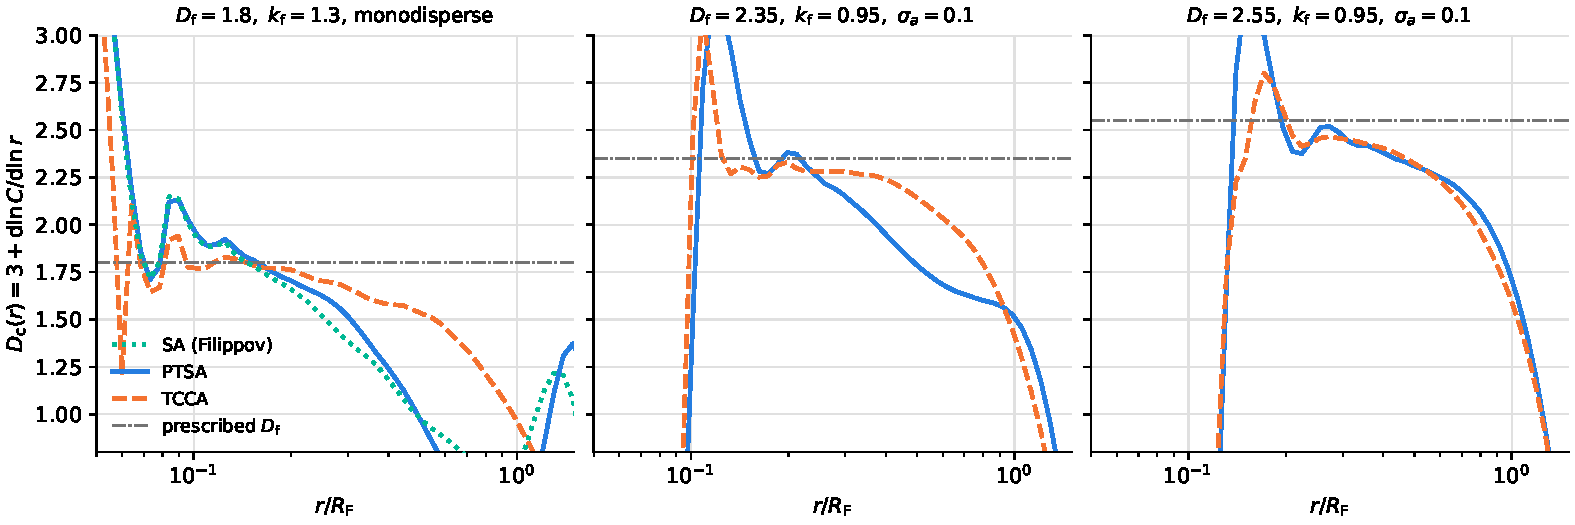
\includegraphics[width=\textwidth]{correlation.pdf}
  \caption{Local correlation dimension $D_\text{c}(r) = 3 + \dd\ln C/\dd\ln r$ of the mean correlation function, from a sliding least-squares fit over 7 logarithmic bins.
  $N_\text{p} = 2048$.
  Left: $\Df = 1.8$, $\kf = 1.3$, equal radii, 40 aggregates per method.
  Centre and right: $\kf = 0.95$, $\sigma_a = 0.10$, 30 aggregates per method (28 for PTSA at $\Df = 2.55$).
  The dash-dotted line is the prescribed $\Df$.
  Values below $r/\RF \approx 0.1$ reflect the discrete structure of touching spheres.}
  \label{fig:correlation}
\end{figure}

\begin{table}[htbp]
  \centering
  \caption{Correlation dimension $D_\text{c}$ fitted to individual aggregates over $r_\text{lo} \le r \le f_\text{hi}\RF$.
  Means $\pm$ standard errors.
  $N_\text{p} = 2048$.}
  \label{tab:correlation}
  \small
  \begin{tabular}{llcccc}
    \toprule
    Case & Method & $[5a, 0.5\RF]$ & $[4a, 0.4\RF]$ & $[5a, 0.7\RF]$ & $[8a, 0.7\RF]$ \\
    \midrule
    $\Df = 1.8$, $\kf = 1.3$ & SA   & $1.62 \pm 0.01$ & $1.74 \pm 0.01$ & $1.51 \pm 0.01$ & $1.37 \pm 0.02$ \\
                              & PTSA & $1.67 \pm 0.01$ & $1.78 \pm 0.02$ & $1.56 \pm 0.01$ & $1.43 \pm 0.02$ \\
                              & TCCA & $1.73 \pm 0.01$ & $1.77 \pm 0.01$ & $1.70 \pm 0.01$ & $1.65 \pm 0.01$ \\
    \midrule
    $\Df = 2.35$, $\kf = 0.95$ & PTSA & $2.14 \pm 0.01$ & $2.24 \pm 0.01$ & $2.03 \pm 0.01$ & $1.88 \pm 0.02$ \\
                                & TCCA & $2.27 \pm 0.01$ & $2.29 \pm 0.01$ & $2.23 \pm 0.01$ & $2.19 \pm 0.01$ \\
    \midrule
    $\Df = 2.55$, $\kf = 0.95$ & PTSA & $2.43 \pm 0.01$ & $2.45 \pm 0.01$ & $2.38 \pm 0.01$ & $2.31 \pm 0.01$ \\
                                & TCCA & $2.43 \pm 0.00$ & $2.44 \pm 0.00$ & $2.38 \pm 0.00$ & $2.31 \pm 0.01$ \\
    \bottomrule
  \end{tabular}
\end{table}

The scripts \texttt{analysis/correlation\_compare.py} and \texttt{analysis/plot\_correlation.py} reproduce Fig.~\ref{fig:correlation} and Table~\ref{tab:correlation}.

Table~\ref{tab:feasibility} shows the range in which TCCA succeeds.
Above $\Df \approx 2.6$ the random search finds no non-overlapping configuration at the required centroid distance.
This agrees with the empirical limit $\kf + \Df \lesssim 3.5$ stated for the C++ code.
PTSA is needed for the compact range.

\begin{table}[htbp]
  \centering
  \caption{Successful TCCA aggregates out of 10 seeds, one try each ($\kf = 0.95$, $\sigma_a = 0.10$).}
  \label{tab:feasibility}
  \small
  \begin{tabular}{lccccc}
    \toprule
    $\Df$ & 1.8--2.5 & 2.6 & 2.7 & 2.8 & 2.9 \\
    \midrule
    $N_\text{p} = 512$  & 10/10 & 10/10 & 3/10 & 0/10 & 0/10 \\
    $N_\text{p} = 2048$ & 10/10 & 9/10  & 0/10 & 0/10 & 0/10 \\
    \bottomrule
  \end{tabular}
\end{table}

Table~\ref{tab:speed} lists the wall time of one successful try.
All times were measured on an i9-14900K while about 30 of its 32 threads were busy.
The ratios are more reliable than the absolute values.
The TCCA time grows with $\Df$ because the clusters must interpenetrate more deeply.

\begin{table}[htbp]
  \centering
  \caption{Wall time per aggregate ($\kf = 0.95$, $\sigma_a = 0.10$, one aggregate per process).}
  \label{tab:speed}
  \small
  \begin{tabular}{rlll}
    \toprule
    $N_\text{p}$ & $\Df$ & PTSA & TCCA \\
    \midrule
    2048   & 2.35 & \SI{13.0}{\second} (mean of 30) & \SI{3.2}{\second} (mean of 30) \\
    2048   & 2.55 & \SI{6.0}{\second} (mean of 30)  & \SI{5.8}{\second} (mean of 30) \\
    21\,720 & 1.8 / 2.0 / 2.35 & not measured & 19 / 13 / \SI{12}{\second} (median of 3) \\
    21\,720 & 2.55 & not measured & \SI{79}{\second} (median of 3, max \SI{140}{\second}) \\
    \bottomrule
  \end{tabular}
\end{table}

%======================================================================
\begin{thebibliography}{9}

\bibitem{thouy1994}
R.~Thouy and R.~Jullien,
A cluster-cluster aggregation model with tunable fractal dimension,
\emph{J.\ Phys.\ A: Math.\ Gen.} \textbf{27}, 2953--2963 (1994).
\href{https://doi.org/10.1088/0305-4470/27/9/012}{doi:10.1088/0305-4470/27/9/012}

\bibitem{singh2020}
A.~K. Singh and E.~Tsotsas,
A tunable aggregation model incorporated in Monte Carlo simulations of spray fluidized bed agglomeration,
\emph{Powder Technol.} \textbf{364}, 417--428 (2020).
\href{https://doi.org/10.1016/j.powtec.2020.02.016}{doi:10.1016/j.powtec.2020.02.016}

\bibitem{singh2021}
A.~K. Singh and E.~Tsotsas,
A fast and improved tunable aggregation model for stochastic simulation of spray fluidized bed agglomeration,
\emph{Energies} \textbf{14}, 7221 (2021).
\href{https://doi.org/10.3390/en14217221}{doi:10.3390/en14217221}

\bibitem{singh2021thesis}
A.~K. Singh,
\emph{Morphology based stochastic simulation of spray fluidized bed agglomeration},
Dr.-Ing.\ thesis, Otto von Guericke University Magdeburg (submitted 2020, defended 2021).

\bibitem{singh2022}
A.~K. Singh and E.~Tsotsas,
Influence of polydispersity and breakage on stochastic simulations of spray fluidized bed agglomeration,
\emph{Chem.\ Eng.\ Sci.} \textbf{247}, 117022 (2022).
\href{https://doi.org/10.1016/j.ces.2021.117022}{doi:10.1016/j.ces.2021.117022}

\bibitem{filippov2000}
A.~V. Filippov, M.~Zurita, and D.~E. Rosner,
Fractal-like aggregates: Relation between morphology and physical properties,
\emph{J.\ Colloid Interface Sci.} \textbf{229}, 261--273 (2000).
\href{https://doi.org/10.1006/jcis.2000.7027}{doi:10.1006/jcis.2000.7027}

\bibitem{skorupski2014}
K.~Skorupski, J.~Mroczka, T.~Wriedt, and N.~Riefler,
A fast and accurate implementation of tunable algorithms used for generation of fractal-like aggregate models,
\emph{Physica A} \textbf{404}, 106--117 (2014).
\href{https://doi.org/10.1016/j.physa.2014.02.072}{doi:10.1016/j.physa.2014.02.072}

\bibitem{moran2019}
J.~Morán, A.~Fuentes, F.~Liu, and J.~Yon,
FracVAL: An improved tunable algorithm of cluster--cluster aggregation for generation of fractal structures formed by polydisperse primary particles,
\emph{Comput.\ Phys.\ Commun.} \textbf{239}, 225--237 (2019).
\href{https://doi.org/10.1016/j.cpc.2019.01.015}{doi:10.1016/j.cpc.2019.01.015}

\bibitem{moteki2019}
N.~Moteki,
``aggregate\_gen'': An efficient C++ code for generating fractal cluster of spheres,
nmoteki/aggregate\_generator (v1.1), GitHub repository (2019).
\href{https://doi.org/10.5281/zenodo.3567236}{doi:10.5281/zenodo.3567236}

\end{thebibliography}

\section*{Acknowledgment}
This document was prepared with the assistance of Claude (Anthropic).
The author assumes full responsibility for the content.

\end{document}
